\section{Experiments} \label{experiments}

During development, the Discovery Service and Specification Retriever software were tested separately by mocking other elements in the Cloudify cluster. This section describes the experiments and their set-ups used to verify that different components integrate and work together flawlessly in a full environment built on real machines. The components in question are the aforementioned Discovery Service and Specification Retriever in addition to Host-Pool Service, Cloudify Manager, Host-Pool Plugin and the test workload, Cloudify Nodecellar Example\cite{Nodecellar}.

\subsection{Hardware set-up}
To verify that the Discovery Service and the Specification retriever function correctly in real environment and on real machines, I set up a test-bed depicted in figure ~\ref{fig:network-venn}.

 \begin{figure}[ht!]
\centering
  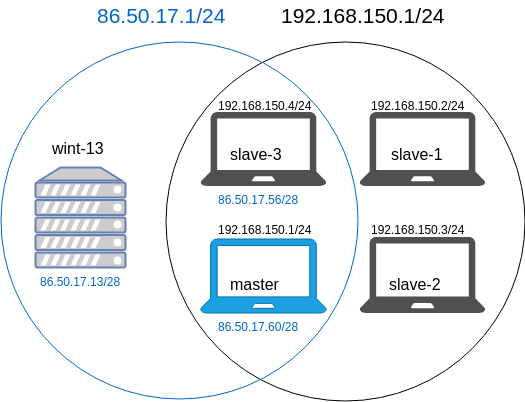
\includegraphics[width=12cm,height=12cm, keepaspectratio]{Network-venn.png}%
  \caption{The testbed hosts are located in a private network but master and slave-3 can also access internet via bastion host wint-13}
  \label{fig:network-venn}
\end{figure}

The test-bed consist of a Lenovo Thinkpad T420S 4173L7G laptop computer with  4-core Intel i5-2540M CPU and 8 GB of RAM acting as a master node in the Cloudify cluster. The three slave-machines are Lenovo Thinkpad Edge E145's with 2-core AMD E1-2500 APU CPUs and 4 GB of RAM. The master host has Centos 7 installed as the operating system to accommodate Cloudify's installation requirements. The three slave machines are running Ubuntu 16.04 as the OS of the slaves can be anything as long as they are Linux-based and the hosts themselves can be accessed via SSH.

\begin{figure}
\centering
  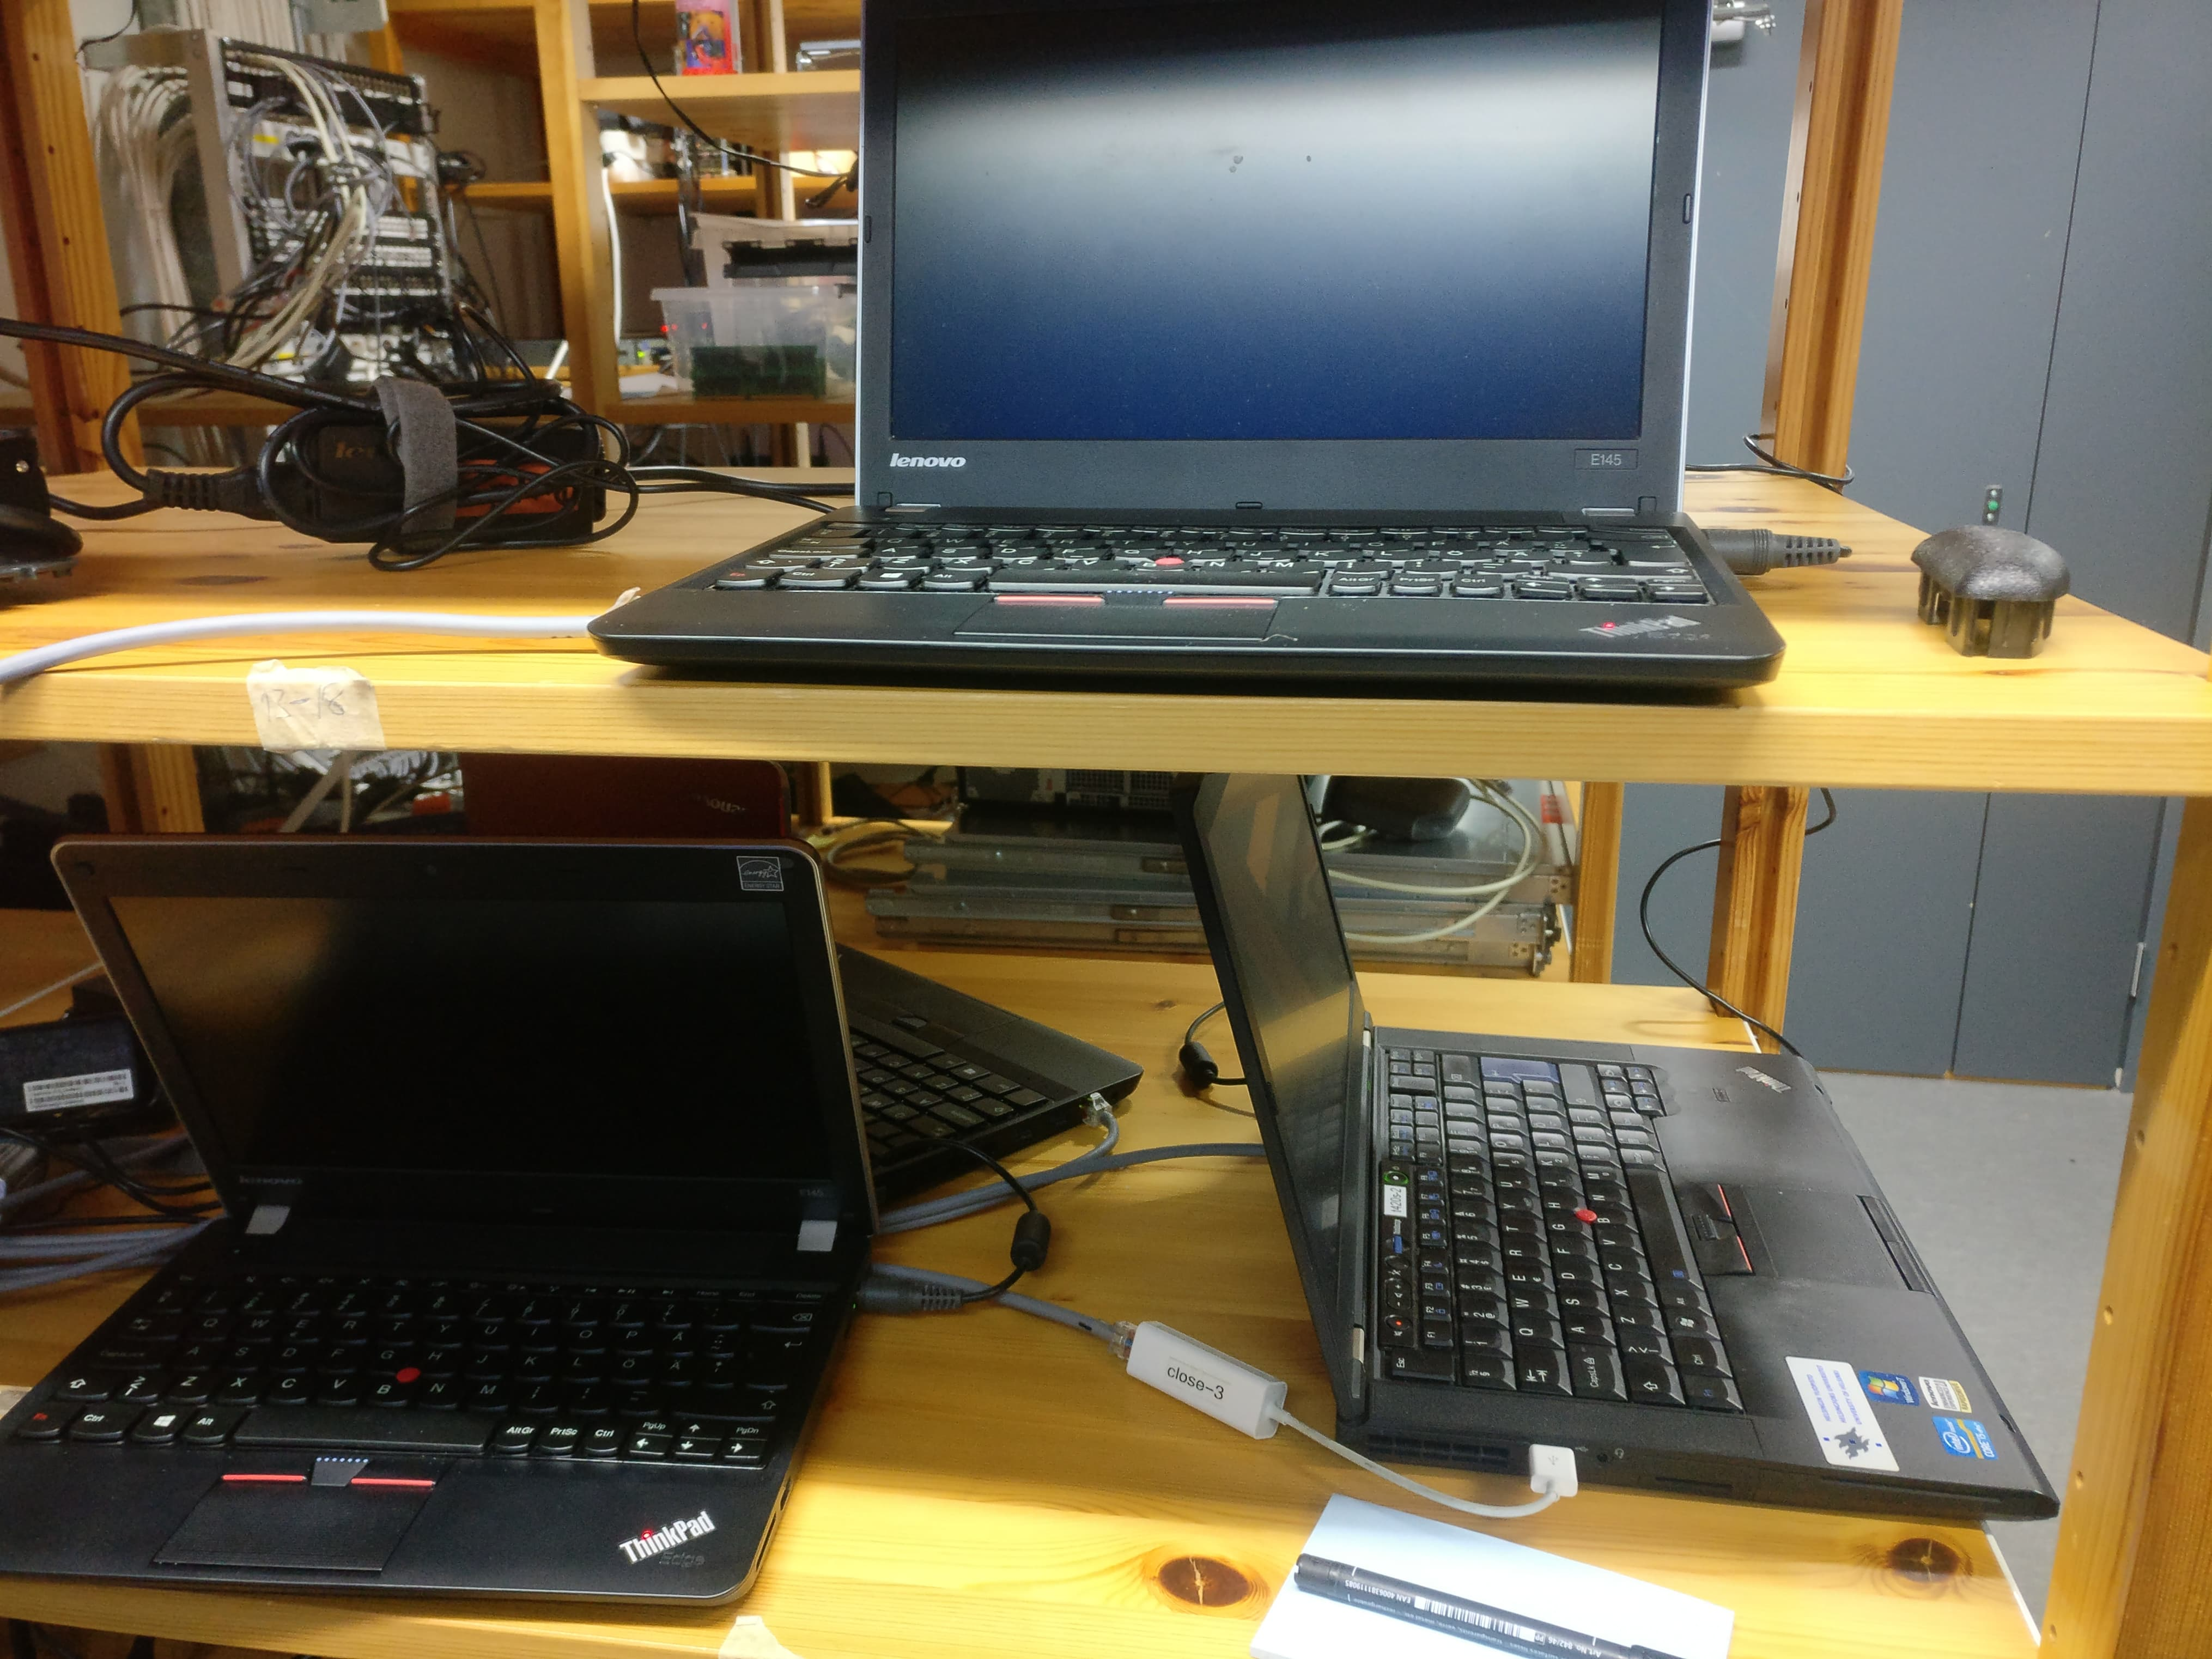
\includegraphics[width=12cm,height=12cm, keepaspectratio]{testbed.jpg}%
  \caption{The actual test-bed. Master node on lower shelf on the right, slaves in the upper and lower shelf}
  \label{fig:test-bed}
\end{figure}

As seen on figure ~\ref{fig:network-venn}, the test-bed set up has two different networks. The Master can be accessed remotely via a bastion host \textit{wint-13}. Wint-13 itself is not a part of the test-bed set up, but it is used to access the testbed remotely and allow internet access for the master host.

Master host has two network interfaces configure for each network it's a part of: The subnet 83.50.17.1 for outside access and 192.168.150.1 which is the subnet dedicated for the Cloudify cluster. Master also serves as a default gateway for all of the slaves. Figure ~\ref{fig:network-venn} shows how slave machines are part of the cluster subnet with static IP addresses. In addition slave-3 is also connected to the 83.50.17.1 subnet. This is to provide a way to drop the host off and connect it back the cluster network but still be able to access it remotely via external network. The physical network is wired with Ethernet cables connected to an HP 5412 zl V2 switch.

\subsection{Software environment set-up}

As mentioned previously, slave hosts do not have many software requirements besides running a Linux distribution as an operating system and having an SSH server installed and accepting connections on the standard port 22. In the test-bed they also have their IP addresses and network interfaces configured statically.

Master node is more intricate than slaves in addition to being more powerful. It has the similar requirements to slaves when it comes to SSH server, but additionally it also runs the following programs:

\begin{itemize}
\item Cloudify Manager
\item Host-pool Plugin within Cloudify Manager
\item Modified Host-pool Service containing Specification Retriever
\item Discovery service
\item Docker
\item Redis running in a Docker container
\end{itemize}

\begin{wraptable}{r}{8cm}
\centering
\begin{tabular}{ | l | p{2cm} | }
\hline
Application & Port \\
\hline
\multicolumn{2}{|c|}{Cloudify ports} \\
\hline
Rest API and UI, HTTP & 80 \\
Rest API and UI, HTTPS & 443 \\
RabbitMQ & 5671 \\
Internal REST communication & 53333 \\
\hline
\multicolumn{2}{| c |}{Other ports} \\
\hline
SSH & 22 \\
Host-pool Service* & 5000 \\
Redis* & 6379 \\
\hline
\multicolumn{2}{| l |}{\textit{* Only internal access}} \\
\hline
\end{tabular}
%\begin{framed}
\caption{Required open ports on the master node. All ports are TCP}
%\end{framed}
\label{table:ports}
\end{wraptable}

In addition the master host has to expose a certain number of ports both internally and externally listed on table ~\ref{table:ports}.

Host-pool plugin runs as a Cloudify deployment managed by Cloudify manager. The modified Host-pool Service runs as a stand-alone Python program listening to port 5000. Even though Cloudify documentation recommends running Host-pool Service as a Cloudify Deployment on a separate host from Cloudify Manager, there are no drawbacks in this kind of local deployment either. 

The Discovery Service is also run as standalone program and it doesn't reserve any ports. However the key-value storage the Discovery Service uses, Redis, is run in a docker container using the official Redis docker image. It reserves the standard  Redis port 6379.

Finally, the server clocks on master host and slave-3 are synchronized with ntp against the ntp server located in the 86.50.17.1/24 cluster network, as synchronized time is needed for accurate measurement results in experiment ~\ref{joining_host}.
  

\subsection{Test cases}

To verify that different parts of the Discovery Service and Specification Retriever work in the real environment, I have come up with five test cases which test how different parts of the software integrate with a real system. First three of the test cases test Discovery Service's ability to monitor  the cluster network and deliver the current cluster status to the Host-pool Service. The fourth test verifies that the Specification Retriever script in the modified Host-pool service collects the hardware data correctly. Finally I am going to run an example workload in the cluster which uses the Discovery Service to manage its logical host-pool. This verifies that the system can be used as an addition to a real Cloudify cluster.

The time measurements from all of the applicable test cases are displayed in table ~\ref{table:measurements}. The table shows the fastest and slowest measured times, average and median times as well as standard deviation. All timed tests are run thirty times and the detailed report of the measurement results can be found in appendix ~\ref{testMeasurements}.

\begin{landscape}
\begin{table}
\centering
\begin{tabular}{ | l || l | l | l | l | l |}
\hline 
Test-case \& Time in seconds & Fastest & Slowest & Average & Median & Standard Deviation \\
\hline \hline
Start-up & 5.402588129 & 5.7881305218 & 5.5874319077 & 5.5766154528 & 0.0941250689 \\
\hline
Joining host & 0.083220005 & 0.2186000347 & 0.1519426159 & 0.1486098766 & 0.0406485995 \\
\hline 
Parting host & 40.3925600052 & 45.1373398304 & 42.5071433465 & 42.4735150337 & 1.3414346833 \\
\hline
Patching a host & 0.0368499756 & 0.0.0572497845 & 0.0481163859 & 0.0482549667 & 0.0044948944 \\ 
\hline
\end{tabular}
\caption{Summary of measurements performed in the test cases}
\label{table:measurements}
\end{table}
\end{landscape}

\subsubsection{Discovering hosts at start up}

As detailed in the section ~\ref{startup}, when Discovery Service is initialised it flushes all of the databases and performs an ARP scan for every IP address in the network. In this experiment I have modified the ARP scanning routine so that it measures the time it takes to scan through the 256 address network. The timing starts when the scan is initialized and stops after the scan. The data stores are reset between every scan.

\subsubsection*{Results}

As seen in the table ~\ref{table:measurements}, scanning through a 256 address network takes approximately 5.6 seconds. This means that it takes approximately 0.022 seconds or 22 milliseconds to send and receive an ARP request for a single host. The real value however varies as the requests may return out of sync and with varying intervals. Also the \verb|timeout| value which denotes the time spent waiting after the last request is set to relatively high value of two seconds.

Overall, all of the runs succeeded and there is no notable deviation in the distribution of times. In comparison to writing and providing host specification in JSON format, automatic scanning is significantly more efficient.

\subsubsection{Detecting a joining host} \label{joining_host}

One of the main features of the Discovery Service is the ability to detect machines joining the network in real time. In this test case Slave-3 is not initially connected to the cluster network. I have prepared a script which first returns a current time stamp on Slave-3 and then enables the network interface facing the cluster network. The sniffer algorithm on the Discovery Service is modified so that it too returns a time stamp upon detecting  a new host. As both hosts are synced against the same time server, the timestamps are comparable allowing me to measure a time it takes for Discovery Service to detect a host after it has joined the network.

\subsubsection*{Results}

As with the start-up scan, the time to detect a joining host is very regular and is more affected by the network speed rather than the implementation overhead. There were however outliers caused by the test implementation. As the network interface on Slave-3 was enabled there was a slight wait in the script execution so that the interface is ready before sending an ARP request. As the script was run multiple times, the ARP cache often did not have time to invalidate and thus no ARP request was automatically sent when the interface was ready. In a real use case, such rapid enabling and disabling of the interface would be unlikely and the cache invalidation a non-issue. In few cases however, the cache was invalidated between a run and the ARP request was sent when interface was ready, causing the Discovery Service to catch the request before the time was recorded on Slave-3 resulting in a negative time in the final results. Those times have been disregarded in the table ~\ref{table:measurements} but are provided in the appendix ~\ref{testMeasurements}.

Overall most of time taken to detect a joining hosts consists of the interval between sending and receiving the ARP request.

\subsubsection{Detecting a departed host}

Similarly to detecting the joining host, detection of a departed host is another major feature of the Discovery Service. The testing procedure is also similar: Slave-3 has a script which drops the host from the network while producing a time stamp for the event. The departure detection in the Discovery Service is modified to return a time stamp when the detection of Slave-3 is detected. The detection is done in the pinger component described in section ~\ref{pinger}, in which a host is declared departed if it fails to reply to a set number of pings. The values for the ping interval and ping failures are five seconds for the interval and three failures. This relatively long interval is likely to cause a wide distribution of time results as the time between Slave-3 getting dropped from the network and the first ping could be five seconds. On the other hand this measurement is representable of a real usage scenario. \newline 

\subsubsection*{Results}

Every execution of the pinging routine consists of two parts which make up the majority of the execution time. First the time out the ARP ping spends waiting for a reply is ten seconds and an interval between pings is five seconds. Depending on how fast a ping routine fires after Slave-3 disconnects, these parts take minimum of forty seconds and maximum of 45 five seconds.

Both extremums are presented in the experiment sampling and both average and median values are close to expected mathematical average. The computational overhead is negligible when compared to the ping interval and time out, but keeping that in mind, the average and median times could have been expected to be slightly over 42,5 seconds. 
Nevertheless, taking into account the expected five second variability of the beginning of execution, another data sample could result in slightly different times but similar standard deviation.

\subsubsection{Patching a host}

Procedure on this test case is similar to the previous two. A script modifies the IP address of Slave-3 from 192.168.150.4 to 192.168.150.5 and back, each modification producing a time stamp for in Slave-3 and each detected address change producing one on Master. Similarly to \textit{Detecting a joining host} experiment, an ARP request is sent manually as the ARP caches may not have time to be invalidated and thus changing the IP address may not trigger an ARP request automatically.

\subsubsection*{Results}

During the preliminary testing it became apparent that in some cases, as one IP address was unused for a longer time than for example in \textit{Detecting a parting host} experiment, ARP caches became invalidated more frequently. This meant, that changing an IP address triggered an automatic ARP call more frequently than first expected and capturing this behaviour required an another time stamp to be recorded in the script on Slave-3. In the experiment, Slave-3 provided time stamp both when the interface was enabled and also when the ARP request was sent manually. The first time stamp prevented negative times in the results but the time itself didn't reflect a time it takes for the Discovery Service to detect and patch an IP change, but rather the time it takes for a the interface to be ready in this particular case. These values have been omitted from the results in table ~\ref{table:measurements} but they are included in the appendix ~\ref{testMeasurements}.

The tests succeeded on every execution. Patching seemed to be the most lightweight of the operations tested: The slowest execution time was circa 26 milliseconds faster than the fastest execution of the \textit{Detecting a joining host} experiment. This is because changing a single field in an existing data object is computationally significantly less demanding than creating a new data object with multiple fields.

Like the results from the previous experiments, \textit{Patching a host} results also indicate correct, fast and regular execution of the routine.

\subsubsection{Retrieving hardware data from the hosts}

This test case shows, that the modified Host-pool Service retrieves correct hardware data from the host. First the hardware data is listed manually on the target host. Next the start-up routine is run which adds all the hosts in the network to logical host pool. The modified Host-pool Service runs the hardware specification retrieval scripts when the hosts are added. Afterwards Host-pool Service can be queried to confirm that correct data was retrieved.

This test case also demonstrates how easily new commands can be added to the Specification Retriever.

\subsubsection*{Results}

Openstack's \textit{Ironic} -project\cite{ironic_troubleshoot} retrieves a modest amount of hardware data, namely the Number of CPUs, available RAM, available disk space and CPU architecture. CPU architecture retrieval was not included in the modified Host-pool Service specification detailed in section ~\ref{specification_retriever}, but to demonstrate specification retrievers capabilities and extendibility, I have added it as well as a command to retrieve the host's graphics card model to the list of commands executed on hosts. The commands are as follows:

\begin{itemize}
\item \verb= lscpu | awk '/Architecture/{ print \$2 }'= which retrieves the cpu architecture.
\item \verb=lscpu | awk '/Model name/' | sed -e 's/Model name://g' -e 's/^[ \t]*//g'= which retrieves the graphics card model while removing whitespace from the command result.
\end{itemize}

In the experiment the additional query commands were added to the modified Host-pool service. Discovery Service was ran normally and the Host-Pool Service REST endpoint was queried for Slave-3's data. Figure ~\ref{fig:master_query} is a screenshot of the query result and it shows the hardware data along with the added CPU architecture and graphics card model. Figure ~\ref{fig:slave_3_specs} is a screenshot showing the same data when queried directly on Slave-3 in remote terminal. The data in Host-pool service query is identical to that queried directly on Slave-3, verifying the correctness of the Hardware Specification retrieval operation. It also verifies, that the Hardware Specification retrieval operation can be easily extended with only minor additions to Host-pool Service.

 \begin{figure}[ht!]
\centering
  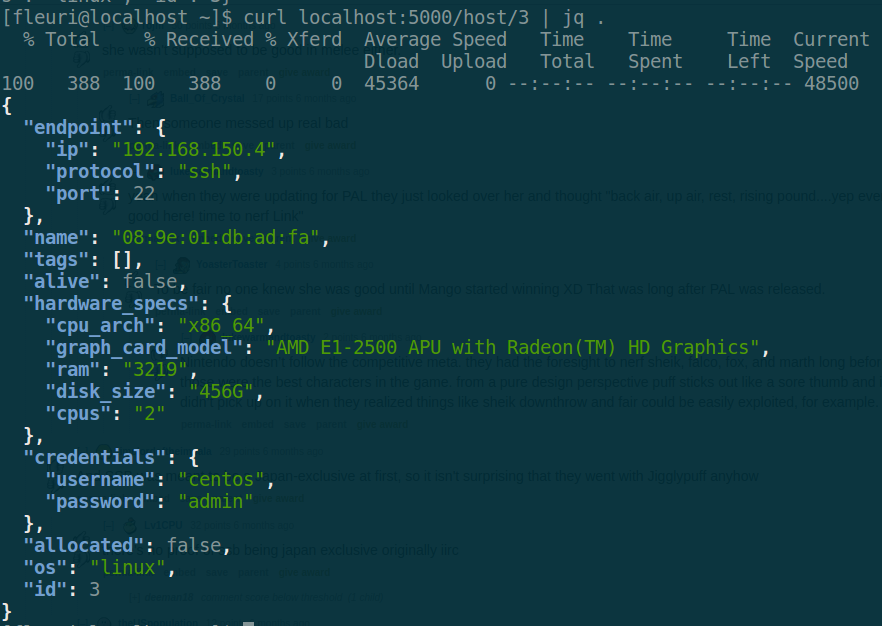
\includegraphics[width=10cm,height=10cm, keepaspectratio]{masterqueryscreenshot.png}%
  \caption{Host-pool service query returns a json with added new fields cpu\_arch and graph\_card\_model}
  \label{fig:master_query}
\end{figure}

 \begin{figure}[ht!]
\centering
  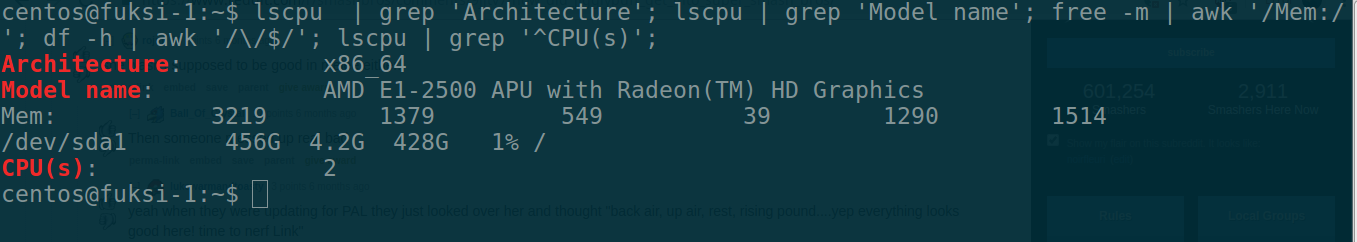
\includegraphics[width=10cm,height=10cm, keepaspectratio]{slave_3_specs_screenshot.png}%
  \caption{The results of individual commands run on Slave-3}
  \label{fig:slave_3_specs}
\end{figure}

\subsubsection{Running an example workload in the system}

The final experiment shows, that Discovery Service works seamlessly when running a real workload in the Cloudify cluster. The workload in question is Cloudify's standard example workload Cloudify Nodecellar Example\cite{Nodecellar}. Nodecellar is a web application which simulates a wine inventory system. It is deployed on two separate hosts with the \textit{nodejs\_host} running a webserver and a Node.js based frontend application whereas the second \textit{mongod\_host} houses MongoDB. The figures ~\ref{fig:console_topology} and ~\ref{fig:console_list} are screenshots of the Cloudify console showing the different components of the Nodecellar deployment and the relations between them. The goal of this experiment is to have a functioning Nodecellar application running on two of the slave hosts which were discovered by the Discovery Service and allocated to Cloudify Manager by the Host-Pool Service.

 \begin{figure}[ht!]
\centering
  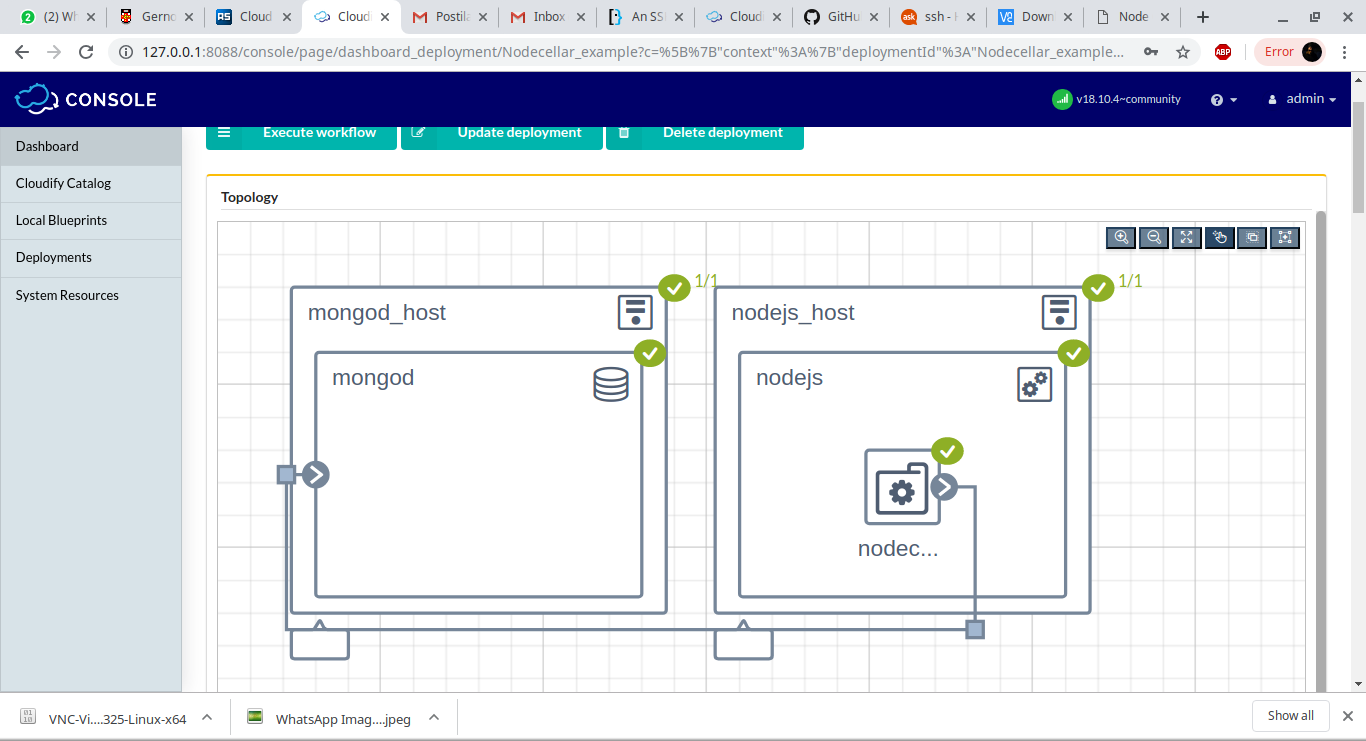
\includegraphics[width=12cm,height=12cm, keepaspectratio]{consoletopology.png}%
  \caption{Cloudify console shows the topology diagram of the Nodecellar deployment}
  \label{fig:console_topology}
\end{figure}

 \begin{figure}[ht!]
\centering
  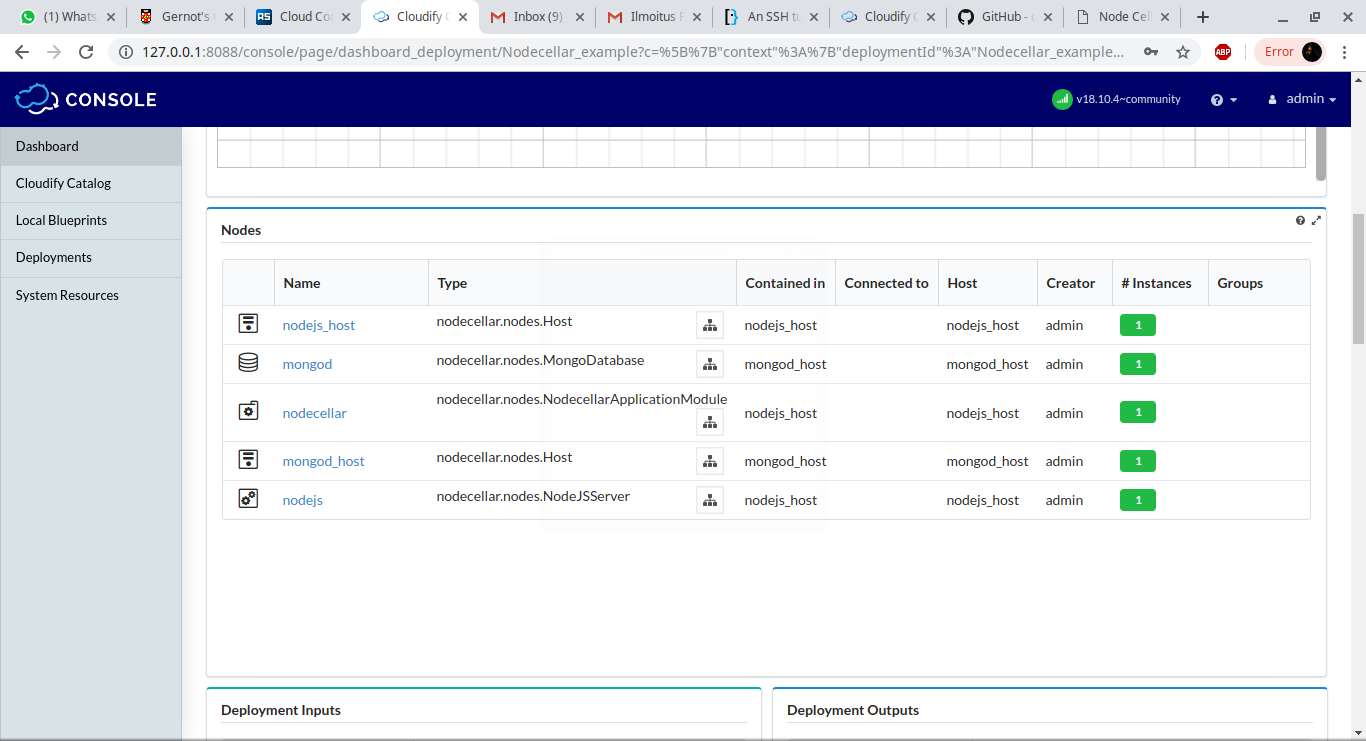
\includegraphics[width=12cm,height=12cm, keepaspectratio]{console_list.png}%
  \caption{Nodecellar deployment's parts listed in the Cloudify console}
  \label{fig:console_list}
\end{figure}

\subsubsection*{Setting up the experiment}

Prior to deploying Nodecellar, I had set up Host-pool Service, Discovery Service and Cloudify Manager. I had also forwarded the port of Cloudify Manager's web console so that I could access it remotely. On Cloudify, every component has to be defined as a Blueprint using TOSCA DSL. When blueprints are uploaded to Cloudify Manager, user can create Deployments of them which in turn create the actual resources.

Before Cloudify Manager could use Host-pool Service to allocate hosts for the deployment, the Host-pool Plugin was required to be installed. The latest version 1.5 was faulty so I downgraded to 1.4. This also meant that I had to manually change Nodecellar Example's blueprint's dependencies to use Host-pool Plugin version 1.4 instead of the default 1.5. After uploading the modified blueprints and creating deployments of them I ran the 'Install' workflow which requested the required hosts from Host-pool Service via Host-pool Plugin and after receiving them installed the required software on them.

\subsubsection*{Results}

As Host-pool Plugin allocates the requested available hosts in order, Slave-1 was designated as the \textit{nodejs\_host} and Slave-2 as \textit{mongod\_host}. To verify that the application is usable and served correctly I forwarded another port via wint-13 bastion host and Master host so that I could  view the web page on my local machine. Figure ~\ref{fig:nodecellar} shows a screenshot of the Nodecellar application. I could also add and remove wines to and from the system as seen on figure ~\ref{fig:chateau}. This validated that the MongoDB database on the second host as well as the connection between the hosts functioned correctly.

Overall it can be concluded that Discovery Service and the modified Host-pool Service function correctly in the experimental scope of this thesis.

 \begin{figure}[ht!]
\centering
  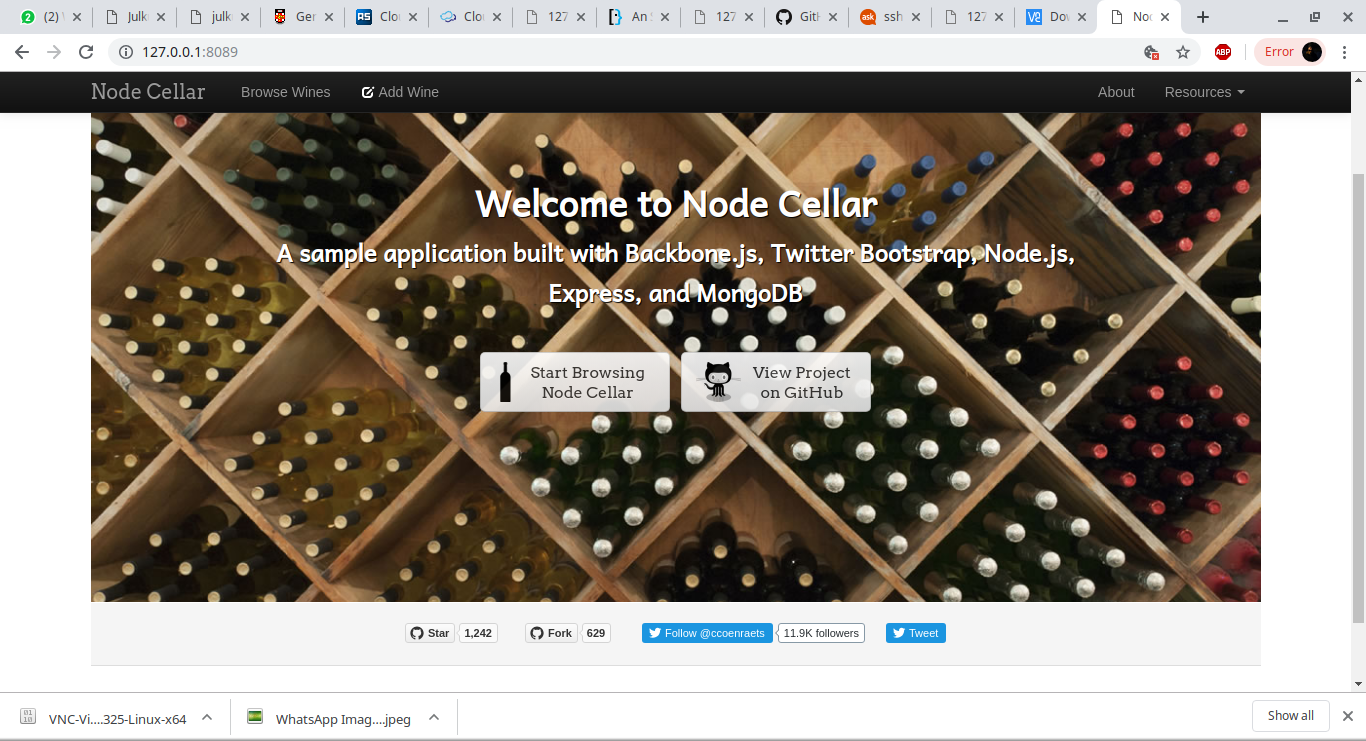
\includegraphics[width=12cm,height=12cm, keepaspectratio]{Nodecellarscreenshot.png}%
  \caption{Cloudify Nodecellar Example's landing page when deployed on the test bed cluster. The localhost IP address is due to port being forwarded to the \textit{node\_js} host.}
  \label{fig:nodecellar}
\end{figure}

 \begin{figure}[ht!]
\centering
  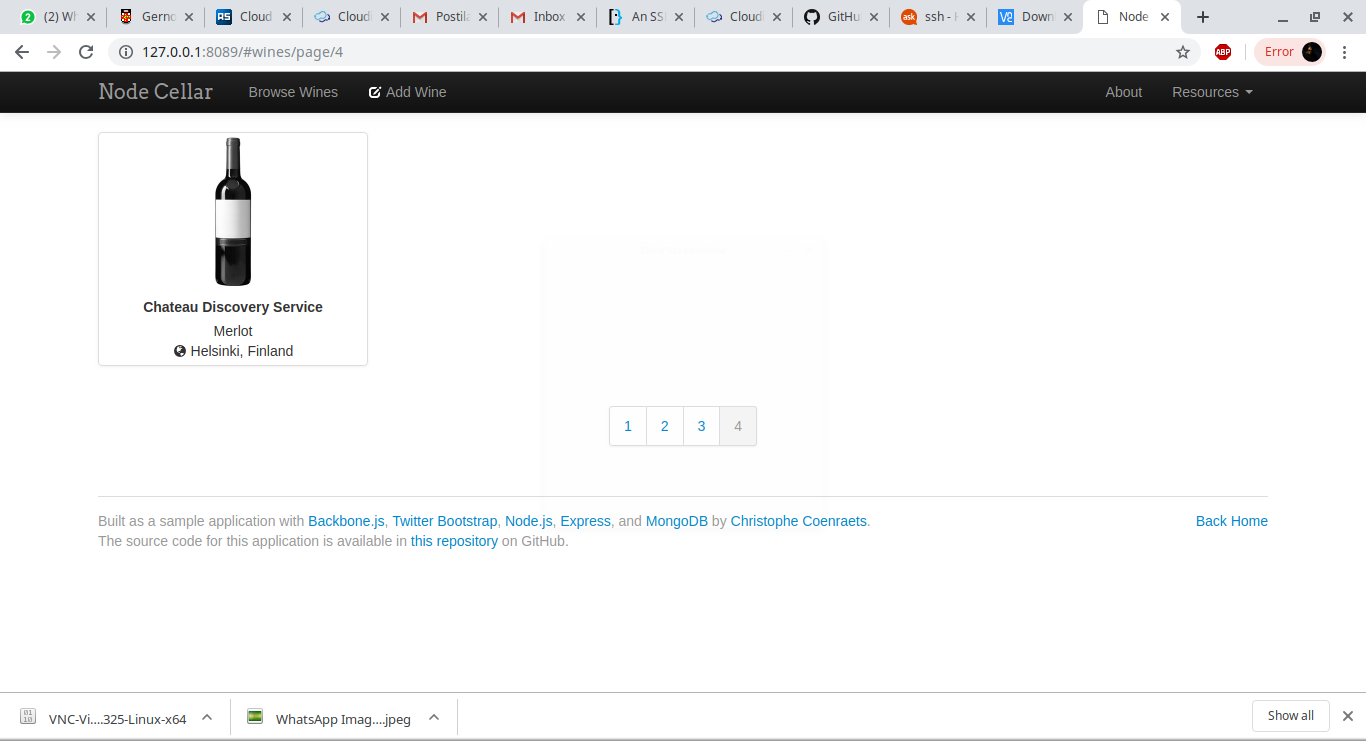
\includegraphics[width=12cm,height=12cm, keepaspectratio]{chateaudiscoveryservice.png}%
  \caption{Nodecellar allows the user to add their own wines to the list. This particular vintage is a real labour of love.}
  \label{fig:chateau}
\end{figure}